\section{Performance}

The HTCC is one of the major CLAS12 systems used in Hall~B experiments with the electron beam. The most
important aspects of the HTCC performance are that it provides good timing, high electron detection efficiency,
and a high rejection factor for charged pions. Each of these parameters is critical for the quality of the data
obtained in experiments since the detector, in combination with the forward electromagnetic calorimeter
\cite{ec-nim}, provides a fast trigger signal for CLAS12. As shown in Section~\ref{htcc-sim-sec}, the MC prediction
for the HTCC detection efficiency for electrons is $\approx$100\%. Figure~\ref{fig:RAFO_2GeV} shows a
distribution of the number of photoelectrons in the HTCC for elastically scattered 2~GeV electrons where the
identification of a negative track as an electron was done based on kinematics. The corresponding thresholds applied
were approximately 2.5 photoelectrons. The measurements were performed using a special procedure with a random
trigger that was not correlated with the HTCC~\cite{trigger-nim}. There were observed 27 events not detected by
the HTCC due to the applied threshold. As shown, the electron detection efficiency is $\eta$ = (99$\pm$0.2)\%,
which is in good agreement with the MC estimate. This result can be considered as a conservative estimate due to
the relatively high threshold used in the measurements.

Elastic electron scattering occurs  at small polar angles.  Inelastic electron scattering covers a much wider range of
polar angles, where the average scattering angles are larger. Such electrons travel longer distance in the radiator
gas (by 10\% to 30\% depending on scattering angle). Consequently the signal strength is higher for these electrons,
and therefore the detection efficiency is higher as compared with the detection efficiency for elastically scattered
electrons.  

\begin{figure}[!ht]
    \centering
    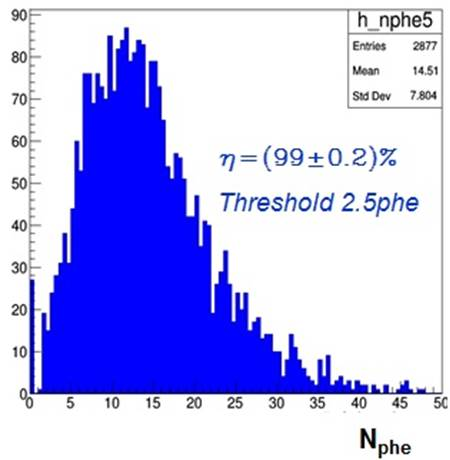
\includegraphics[width=1.0\linewidth,trim={0.0cm 0.0cm 0.0cm 0.0cm},clip]{images/RAFO_2GeV.jpg}
    \caption{Electron detection efficiency for elastically scattered electrons at 2~GeV. Data are obtained with the
      random trigger not correlated with the HTCC or other detector components of CLAS12.}
    \label{fig:RAFO_2GeV}
\end{figure}

Figure~\ref{fig:positivePNPEC6595} shows the response of the detector over a wide range of particle momenta.
The increase in the number of events at high momentum ($>$5~GeV) is due to registration of charged pions (above
threshold for their registration in the HTCC) and this is clearly illustrated.

\begin{figure}[!ht]
    \centering
    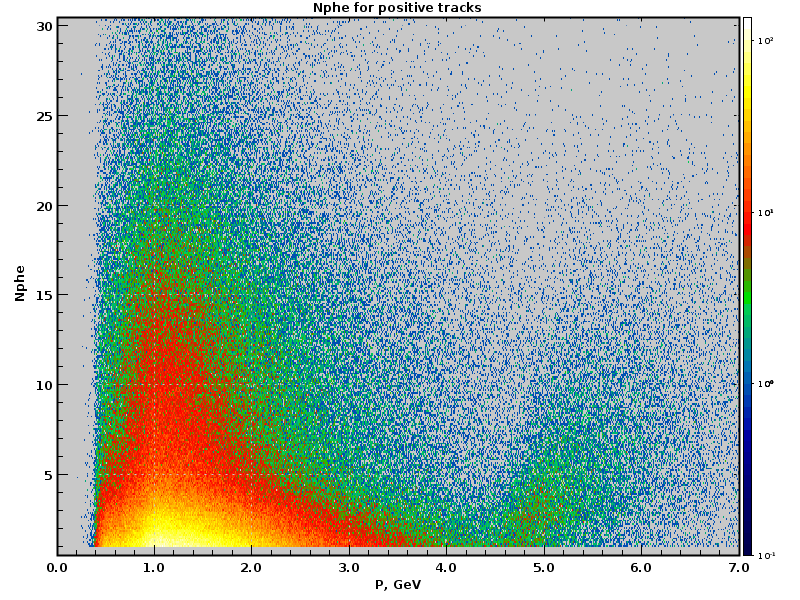
\includegraphics[width=1.0\linewidth,trim={0.0cm 0.0cm 0.0cm 0.0cm},clip]{images/positivePNPEC6595.png}
    \caption{Distribution of the HTCC response in terms of the number of photoelectrons vs. momentum over a wide
      momentum range, including the region beyond the threshold of charged pion registration ($>$5~GeV). The data
      were obtained for positrons and $\pi^+$-mesons.}
    \label{fig:positivePNPEC6595}
\end{figure}

The signal strength in the HTCC depends on the actual properties of the mirror facets, such as their final shape
and reflectance. The accuracy of the combined mirror assembly, the alignment of the HTCC components (mirror,
PMTs, Winston cones), and the composition of the radiator gas, all influence the final results. The FADC histogram of
the typical signal strength distribution obtained in half-sectors \#1 and \#2 of sector~1 is shown in
Fig.~\ref{fig:Signal_S1_HS1_HS2_R1_R2}. The signal strength for scattered electrons averaged over all HTCC
channels is shown in Fig.~\ref{fig:Average_HTCC_Signal}. The experimentally measured mean value of 16.3
photoelectrons is close to the Monte Carlo simulation results (see Fig.~\ref{fig:10cm_Targ_5T_Field_Phi}).

\begin{figure}[!ht]
    \centering
    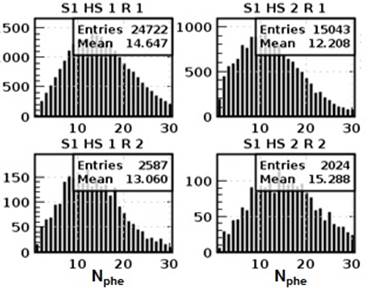
\includegraphics[width=1.0\linewidth,trim={0.0cm 0.0cm 0.0cm 0.0cm},clip]{images/Signal_S1_HS1_HS2_R1_R2.jpg}
    \caption{Typical distributions of the signal strength in channels covering polar angles in the range of $5^\circ$ to
      $12.5^\circ$ (Ring~1) and $12.5^\circ$ to $20.0^\circ$ (Ring~2) within an azimuthal interval of $60^\circ$.}
    \label{fig:Signal_S1_HS1_HS2_R1_R2}
\end{figure}

\begin{figure}[!ht]
    \centering
    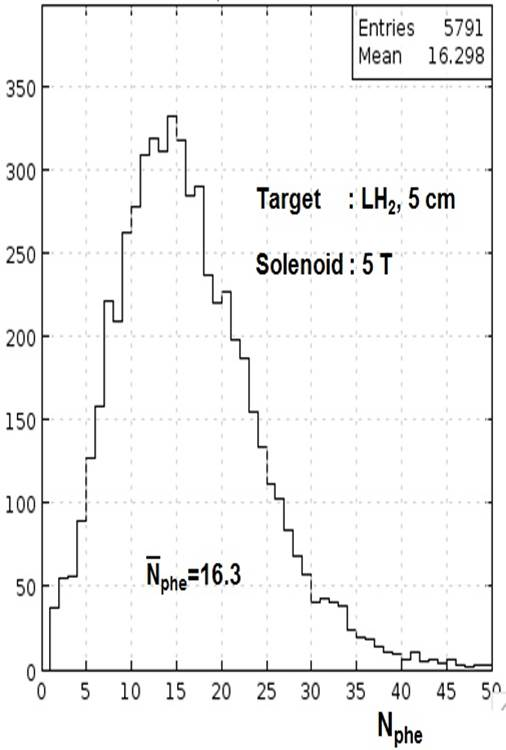
\includegraphics[width=1.0\linewidth,trim={0.0cm 0.0cm 0.0cm 0.0cm},clip]{images/Average_HTCC_Signal.jpg}
    \caption{The HTCC average signal strength for electrons from beam data at 10.6~GeV.}
    \label{fig:Average_HTCC_Signal}
\end{figure}

Figure~\ref{fig:HTCC_Response_run4013} shows the uniformity of the HTCC response for different electron
momenta. Fig.~\ref{fig:avgNPE_Theta_Phi_Dev_Build-2_NO_HOLES}  shows the distribution of the HTCC response
over the entire face of the mirror in the $xy$ (transverse) plane. 

The data show that the integrated signal strength is about 16.5 photoelectrons. At large electron polar scattering
angles in range of 27.5$^\circ$ to 35$^\circ$, the statistics are lower.
Figure~\ref{fig:statistics_Theta_Phi_Dev_Build_NO_HOLES} shows the distribution of statistics in all 6 sectors. 

\begin{figure}[!ht]
    \centering
    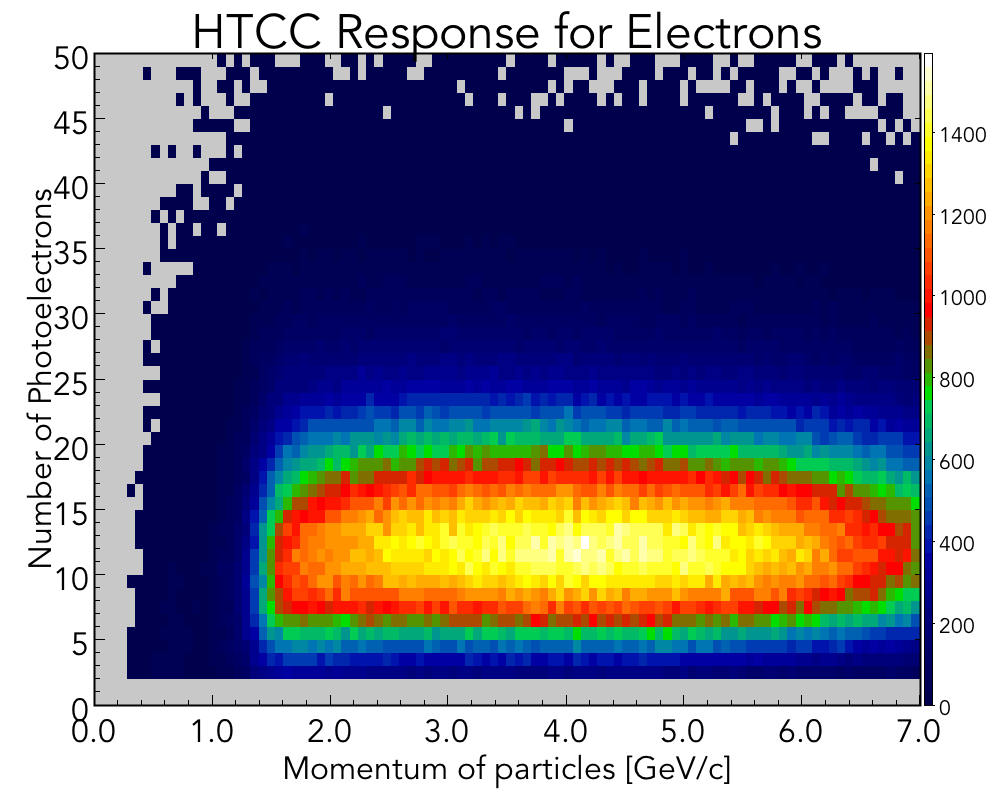
\includegraphics[width=1.0\linewidth,trim={0.0cm 0.0cm 0.0cm 1.73cm},clip]{images/HTCC_Response_run4013.png}
    \caption{The HTCC response for electrons: signal strength vs. momentum at 10.6~GeV electron beam energy.}
    \label{fig:HTCC_Response_run4013}
\end{figure}

\begin{figure}[!ht]
    \centering
    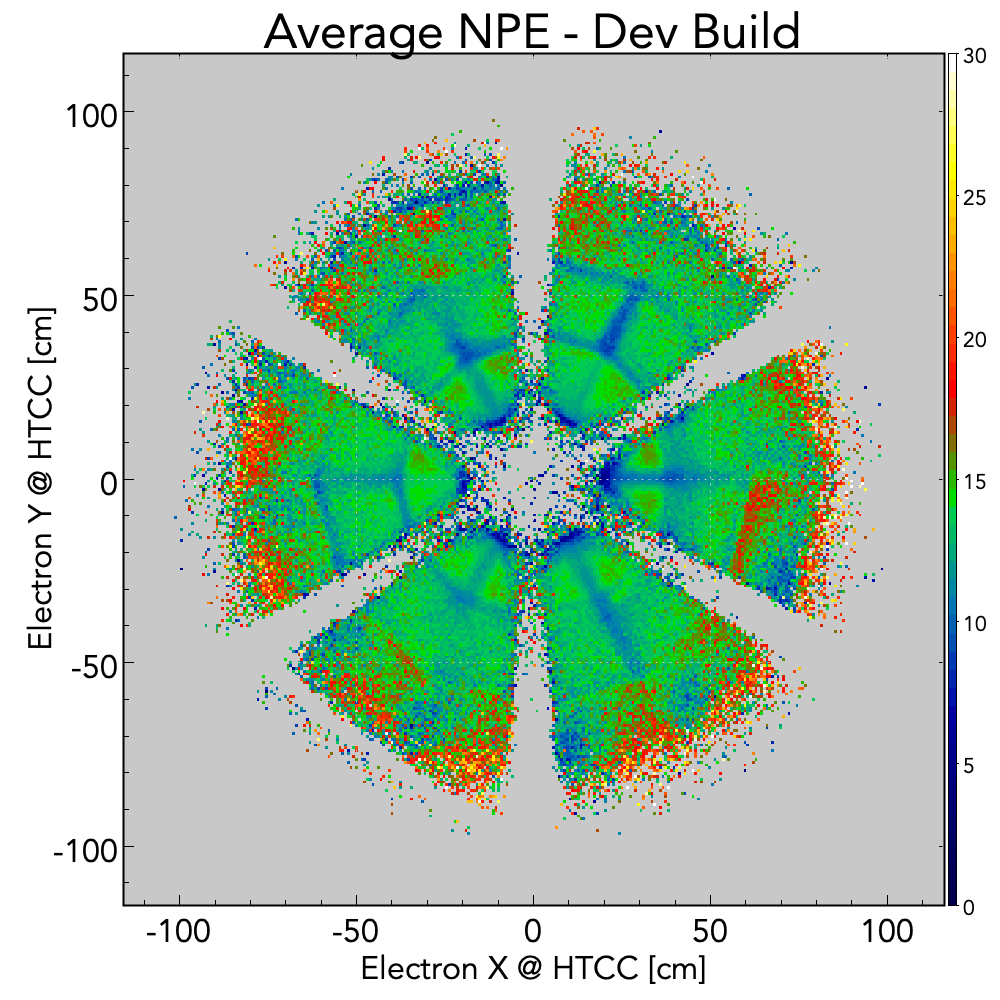
\includegraphics[width=1.0\linewidth,trim={0.0cm 0.0cm 0.0cm 1.67cm},clip]{images/avgNPE_Theta_Phi_Dev_Build-2_NO_HOLES.png}
    \caption{The HTCC response (in terms of the number of photoelectrons) for electrons in the $xy$-plane of the
      mirror.}
    \label{fig:avgNPE_Theta_Phi_Dev_Build-2_NO_HOLES}
\end{figure}

\begin{figure}[!ht]
    \centering
    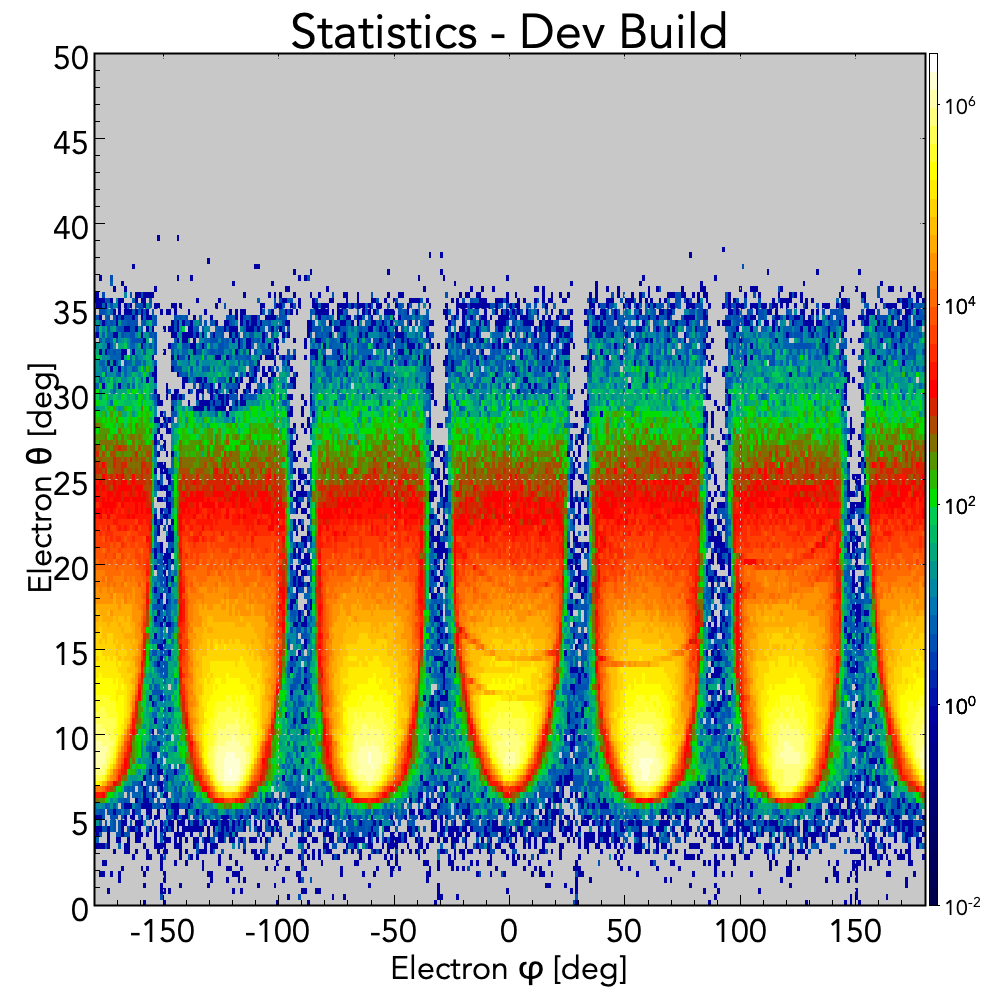
\includegraphics[width=1.0\linewidth,trim={0.0cm 0.0cm 0.0cm 1.67cm},clip]{images/statistics_Theta_Phi_Dev_Build_NO_HOLES.png}
    \caption{Distribution of statistics in terms of electron polar angle vs. azimuthal angle in all 6 of the CLAS12
      Forward Detector sectors.}
    \label{fig:statistics_Theta_Phi_Dev_Build_NO_HOLES}
\end{figure}

We also note that in cases when the electrons cross a mirror close to its edges (at approximately at 5$^\circ$ and
35$^\circ$) one should expect unavoidable losses in the signal strength: some part of the Cherenkov light just passes
by the mirror. As far as the internal borders between adjacent mirrors are concerned, there are similar losses that
take place and are finally partially compensated due to the complete azimuthal symmetry of the detector, see
Fig.~\ref{fig:avgNPE_Theta_Phi_Dev_Build-2_NO_HOLES}. The width of the area along the internal boundaries that
is deformed in the direction normal to the mirror face due to the shrinkage of the glue is estimated to be between
$\sim 5 - 10$~mm. This area includes the technological zone of width $\sim$0.5~mm that does not reflect the light at
all. As a result these regions (width up to $\sim$10~mm) along the internal boundaries between the mirror facets
defuse the light impinging on the area, and therefore the signal strength is reduced. This edge effect is expected
given the design of the detector.
